\chapter{Limits}

\section{Behaviors at infinity: asymptotes and rational functions}

Polynomials are very well behaved, in a sense that if $f(x)$ is a polynomial, the only way that $f(x) \appr \infty\infty$, is that $x \appr \pm\infty$. However, there are other family of functions which can have infinities anywhere that it likes: the \textbf{rational functions}.\index{rational functions}

A rational function $F(x)$ is a function that can be written as a ratio of two polynomials:
\begin{equation}
	F(x) = \frac{P(x)}{Q(x)} = \frac{p_0 + p_1x^1 + \dots + p_nx^n}{q_0 + q_1x^1 + \dots + q_mx^m}.
\end{equation}
By the fundamental theorem of algebra, we can always factor these polynomials into
\begin{equation}
	\begin{multlined}
		P(x) = (x - P_0)(x - P_1)\dots(x - P_n), \\
		Q(x) = (x - Q_0)(x - Q_1)\dots(x - Q_n),
	\end{multlined}
\end{equation}
where $P_0, \dots, P_n, Q_1, \dots, Q_n$ are components of the complex plane; thus,
\begin{equation}
	F(x) = \frac{(x - P_0)(x - P_1)\dots(x - P_n)}{(x - Q_0)(x - Q_1)\dots(x - Q_n)}.
\end{equation}
When $x$ approaches any of the $Q$'s in the denominator, $Q(x) \appr 0$, and thus $F(x) \appr \infty$ there. The point $x = Q_1, Q_2, \dots, Q_n$ are called the \textbf{singularities} of $F(x)$.

For example, the function $F(x) = \frac{1}{x}$, sketched in \cref{fig:reciprocal-function} explodes to $\pm\infty$ at $x \appr 0$, but gradually decreases to $0$ when $x \appr \pm\infty$. To study these functions, we have to define a line called the \textbf{asymptote}.
\begin{figure}[ht]
	\centering
	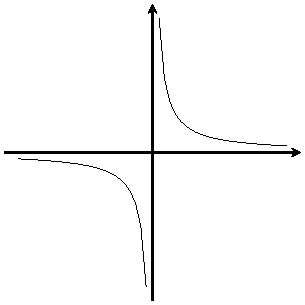
\includegraphics{geometryandcalculus/reciprocal-function.pdf}
	\caption{Graph of $\frac{1}{x}$}
	\label{fig:reciprocal-function}
\end{figure}

An \textbf{asymptote} is a line that the graph of a function approaches but never intersect. E.g., the function $F(x) = \frac{1}{x}$ has two asymptotes: the line that runs through the $x$ axes, and the line that runs through the $y$-axis. Generally, an asymptote could be horizontal, vertical, or even slanted.

